

\section{AIS - Automatic Identification System}

The Automatic Identification System (AIS) is an automated tracking system used by vessels for identifying and locating ships. By electronically exchanging data with other nearby ships, AIS base stations, and satellites, it provides a real-time digital picture of maritime traffic, which is essential for collision avoidance and maritime domain awareness.

\subsection{Transmission Mechanism}

AIS operates in the VHF maritime band. It primarily uses two dedicated frequencies to manage high traffic volume and prevent signal interference:

\begin{itemize}
    \item AIS 1: 161.975 MHz
    \item AIS 2: 162.025 MHz
\end{itemize}

Because AIS is a brodcast system, it is inherently unidirectional and does not require a handshake or connection establishment. Each vessel continuously transmits its information, which can be received by any nearby AIS-equipped receiver within range.

To prevent collisions of messages in busy areas, AIS uses a dynamic slot allocation mechanism. Each vessel monitors the channel and selects an available time slot for its transmission. If a vessel detects that its chosen slot is occupied, it will randomly select another slot, ensuring efficient use of the VHF spectrum even in congested maritime environments.

Reporting intervals for AIS transmissions vary based on the vessel's status and speed, as defined in ITU-R M.1371-5. For example, a vessel at anchor may transmit every 3 minutes, while a vessel underway at high speed may transmit every 2 seconds. This adaptive reporting ensures that information is updated more frequently when the vessel is in motion or changing course, while conserving bandwidth when stationary.

\begin{table}[h!]
\centering
\caption{AIS Reporting Intervals for Shipborne Mobile Equipment (ITU-R M.1371-5)}
\label{tab:ais_reporting_rates}
\begin{tabular}{|l|l|l|}
\hline
\textbf{Vessel Status / Speed} & \textbf{Class A (SOTDMA)} & \textbf{Class B (CS/SO)} \\ \hline
At anchor or moored & 3 min & 3 min \\ \hline
At anchor or moored & 10 s & 3 min \\ \hline
0--14 knots & 10 s & 30 s \\ \hline
0--14 knots (changing course) & 3 1/3 s & 30 s \\ \hline
14--23 knots & 6 s & 15 s \\ \hline
14--23 knots (changing course) & 2 s & 15 s \\ \hline
$>$ 23 knots & 2 s & 5 s \\ \hline
$>$ 23 knots (changing course) & 2 s & 5 s \\ \hline
Static Information & Every 6 min & Every 6 min \\ \hline
\end{tabular}
\end{table}


\vspace{0.5cm}

Range of system is typically 20 to 30 nautical miles, depending on antenna height and atmospheric conditions. There is a satellite variant of AIS, known as S-AIS, which allows for global coverage by receiving signals from space, but this is not the focus of this project.

\subsection{Data Transmitted}
\label{subsection:data_tx}

The information broadcast by an AIS transponder is categorized into three types:

\begin{itemize}
    \item \textbf{Static Information:} Ship name, IMO number, call sign, vessel type, and vessel dimensions (programmed at installation).
    \item \textbf{Dynamic Information:} Automatically updated data including GPS position, Course Over Ground (COG), and Speed Over Ground (SOG).
    \item \textbf{Voyage-Related Information:} Destination, estimated time of arrival (ETA), and current draught (entered manually by the crew).
\end{itemize}


\subsection{Vessel Type Classification}

\begin{longtable}{clcl}
\caption{AIS Vessel Type Codes (ITU-R M.1371)} 
\label{tab:ais-vessel-types} \\
\toprule
\textbf{Code} & \textbf{Vessel Type} & \textbf{Group} & \textbf{Notes} \\
\midrule
\endfirsthead
\multicolumn{4}{c}{\tablename\ \thetable{} -- continued} \\
\toprule
\textbf{Code} & \textbf{Vessel Type} & \textbf{Group} & \textbf{Notes} \\
\midrule
\endhead
\midrule
\multicolumn{4}{r}{\textit{Continued on next page}} \\
\endfoot
\bottomrule
\endlastfoot

0   & Not available             & Unknown  & Default / not specified \\
\midrule
\multicolumn{4}{l}{\textit{Special Purpose Ships}} \\
\midrule
01  & Science / Research vessel & Special  & \\
02  & Training vessel           & Special  & \\
03  & Government-owned vessel   & Special  & \\
04  & Ice breaker               & Special  & \\
05  & Buoy / AtoN tender        & Special  & Aids to Navigation \\
06  & Cable layer               & Special  & \\
07  & Pipe layer                & Special  & \\
09  & Special purpose ship      & Special  & No additional information \\
\midrule
\multicolumn{4}{l}{\textit{Support Vessels}} \\
\midrule
11  & FPSO vessel               & Support  & Production, Storage \& Offloading \\
12  & Fish factory ship         & Support  & \\
14  & Offshore support vessel   & Support  & \\
17  & Construction vessel       & Support  & \\
18  & Crew boat                 & Support  & \\
19  & Support vessel            & Support  & No additional information \\
\midrule
\multicolumn{4}{l}{\textit{Wing in Ground / Fishing / Special}} \\
\midrule
20  & Wing in ground (WIG)      & WIG      & \\
30  & Fishing                   & Fishing  & \\
31  & Towing                    & Tug/Tow  & \\
33  & Dredging / underwater     & Special  & \\
34  & Diving operations         & Special  & \\
35  & Military operations       & Military & \\
36  & Sailing                   & Sailing  & \\
37  & Pleasure craft            & Pleasure & Recommended for USV/drone \\
\midrule
\multicolumn{4}{l}{\textit{High Speed Craft}} \\
\midrule
40  & High speed craft (HSC)    & HSC      & All ships of this type \\
\midrule
\multicolumn{4}{l}{\textit{Special Craft}} \\
\midrule
50  & Pilot vessel              & Special  & \\
51  & Search and rescue         & Special  & SAR \\
52  & Tug                       & Tug/Tow  & \\
53  & Port tender               & Special  & \\
54  & Anti-pollution            & Special  & \\
55  & Law enforcement           & Special  & \\
58  & Medical transport         & Special  & \\
59  & Non-combatant ship        & Special  & Per RR No.\ 18 \\
\midrule
\multicolumn{4}{l}{\textit{Passenger / Cargo / Tanker / Other}} \\
\midrule
60  & Passenger                 & Passenger & All ships of this type \\
70  & Cargo                     & Cargo     & All ships of this type \\
80  & Tanker                    & Tanker    & All ships of this type \\
90  & Other                     & Other     & All ships of this type \\

\end{longtable}

\noindent\textbf{Note:} Codes x1--x4 denote hazardous cargo categories A--D, omitted for brevity.
Codes 01--19 are an extended classification outside the core ITU-R M.1371 range (20--99).\\[4pt]
\noindent\textbf{Drones / USV:} No dedicated code exists.
Use \textbf{37} (civilian), \textbf{35} (naval), or \textbf{90} (unambiguous).




\subsection{AIS Vulnerability: GPS Integration and Spoofing}

The integrity of AIS data is fundamentally dependent on the Global Navigation Satellite System (GNSS), most commonly GPS. While AIS uses VHF for the transmission of data, the "Dynamic Information" (position, speed, and course) is pulled directly from the ship’s onboard GPS receiver. This creates a critical vulnerability: if the GPS signal is compromised, the AIS broadcast becomes a vehicle for misinformation.



\begin{figure}[htbp]
    \centering
    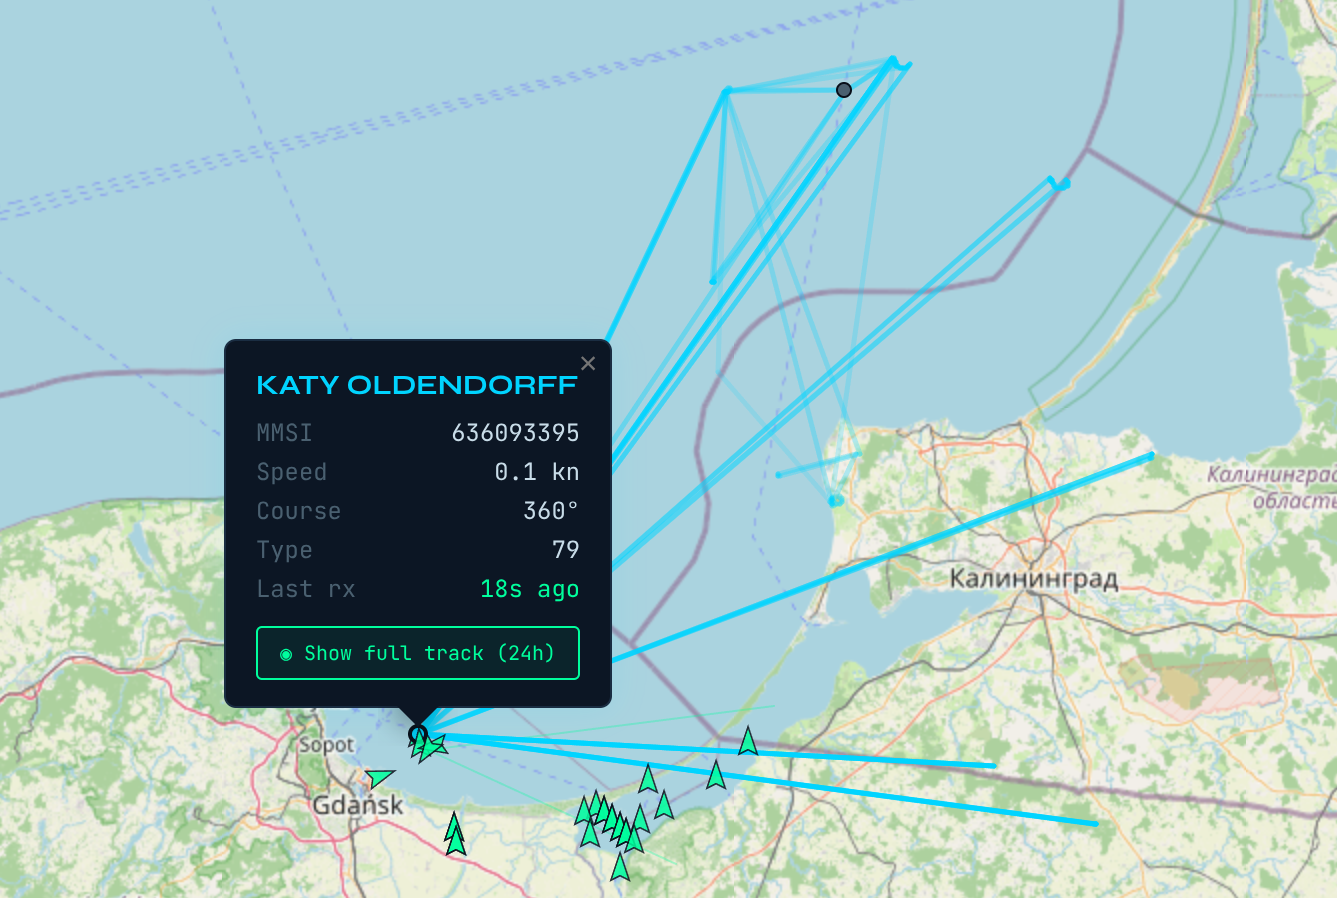
\includegraphics[width=0.6\textwidth]
    {images/AIS_GPS_SPOOF.png}
    \caption{GPS spoofing attack on a vessel, showing the compromised GPS signal.}
    \label{fig:spoofed_GPS}
\end{figure}



\subsection{Synthetic and Virtual AIS Aids to Navigation (AtoNs)}
A significant development in modern maritime infrastructure is the use of AIS signals to represent physical objects without placing electronics on the objects themselves. This is achieved through Synthetic and Virtual AIS AtoNs, which use the 99 prefix MMSI format (specifically \textbf {99MID1XXX} or \textbf {99MID6XXX}) to distinguish them from vessels.

\textbf {Synthetic AIS AtoNs}
A Synthetic AIS AtoN exists where there is a physical buoy or structure in the water, but it does not have its own AIS transmitter. Instead, a nearby AIS shore station (Base Station) broadcasts an AIS Message 21 that contains the exact coordinates of that physical buoy. This provides the mariner with a digital icon on their ECDIS/Radar that correlates with the physical object they see through the window, without the cost or maintenance of installing batteries and transmitters on every buoy.

\textbf {Virtual AIS AtoNs}
Unlike the synthetic version, a Virtual AIS AtoN marks a point where no physical buoy exists.

These are critical for "Time-Critical" marking. If a vessel sinks in a busy channel or a new hazard is discovered, authorities can instantly broadcast a Virtual AtoN to warn ships before a physical buoy can be deployed.
